\documentclass[../ClassicThesis.tex]{subfiles}
\begin{document}

%************************************************
\chapter{Joint Computation}\label{ch:joints}
%************************************************

% Use active Voice (we do….)
% Ein Gedanke pro Paragraph
% Terminologie anpassen über alle Arbeiten hinweg (was ist eine Plate für alle…)
% Jeder sollte eine kleine Related Work section haben
% Erklärungen zu warum dieser Algorithmus genutzt wurde und nicht ein anderer + limitations des gewählten Algorithmus
% Hübsche Bildchen zum anschaulichen Erklären!! (ebenfalls konsistent halten: gleich geformte labels etc.)

\section{Joint computation}
TODO: buy green and orange (or at least two different colors) of acrylic for demo objects and pictures in the paper

\subsection{Volume based clipping}
\paragraph{prerequisite: plategraph intersection lines}
As seen before in the step [plateGraph] up to four intersectionlines will have been calculated.\\
Two of them lie both on one side of the plate and the other two belong to the second side. The two lines on one side build a rectangle when their ends are connected. We use those two rectangles to cut out of the plate what will get fingerjoints.\\
TODO: Insert image of the four lines, with the two rectangles marked.


\subsection{Female Joint Computation}
\subsection{Male Joint Computation}

\subsection{Different Fingerjoint types}
TODO: Bilder noch so anpassen, dass nur females/males zu sehen und in echt, wie sie zusammen stecken
\subsubsection{Fingerjoint template}
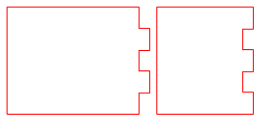
\includegraphics[width=0.5\columnwidth]{Images/fingerjoints.png}
\paragraph{How these joints look like}
\paragraph{How these joints work, and for what material}

\subsubsection{JimJoint template}
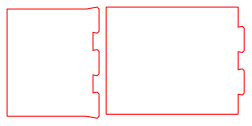
\includegraphics[width=0.5\columnwidth]{Images/jimjoints.png}
\paragraph{How these joints look like}
\paragraph{How these joints work, and for what material}
paper or other easily bendable/eindrueckbar material

\subsubsection{Schwalbe template}
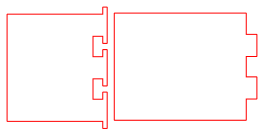
\includegraphics[width=0.5\columnwidth]{Images/schwalbe.png}
\paragraph{How these joints look like}
\paragraph{How these joints work, and for what material}

\subsection{adjusting fingerjoints length when plates are angled}
\paragraph{Deus?}

\subsection{Alternative solutions}


\section{Future work}

\end{document}